




\begin{lemma}\label{l:consistencyEndGBS}



Let  and  be the parameters for each of the  failure models Mi as reported in Table \ref{t:parameters} and used by the algorithm in Fig. \ref{fig:server}-\ref{fig:client}.
Let  for each failure model Mi considered. 
At the end of each round, at least  correct servers store the same value  in their  local variable.
\end{lemma}

\begin{proofL}
Each non-faulty server updates its  local variable at the end of each round  (i) in line  \ref{s21} i.e., if there exists at least a pair in the  local variable, or (ii) in line  \ref{s23} i.e.,  is empty and there exist at least  same values in .


First we prove that one of the two cases always happens and then we prove that the number of non-faulty servers storing the same values  is .
The  local variable is initialized by any non-faulty server  to  at the beginning of each round  (cfr. line \ref{s2}) and it is updated when a {\sc write} message is received by \footnote{Recall that such {\sc write} message is sent by the writer client in the send phase of the first round starting after the  invocation and it is delivered by any non-faulty server in the same round.}.
Thus, case (i) corresponds to a scenario where at least a  operation is executed in round  and case (ii) corresponds to a scenario where no  is running.

\begin{itemize}
\item {\bf Case (i):}  In this case the claim simply follows by considering that (i) writer clients broadcast a {\sc write} message in the send phase of round , (ii) clients are correct so the same set of values is delivered to all servers that will apply a deterministic function to select the value  and (iii) at most  servers are faulty and may skip the update of their  variable.\\

\item {\bf Case (ii):}  {\bf and line \ref{s22} is true.} In this case, the  variable is updated according to the values stored in . Such variable is emptied by every non-faulty process at the beginning of each round (cfr. line \ref{s1}) and is filled in when an {\sc echo} message is delivered.
Such message is sent at least by any server, believing it is correct, at the beginning of each round.
Let  be the round in which the last  operation terminated. Note that, due to above hypothesis, a  operation always exists as we assume a fictional write happening instantaneously at round . Without loss of generality, let us consider the round .
Due to case (i), at the end of , at least  non-faulty servers store the same value  in their local variable .
Thus, at the beginning of , at least  correct servers will send an {\sc echo} message, where  is the number of non-faulty processes that become faulty while passing from  to  (i.e.  for all the models but Burhman's one where  as faulty processes move during the send phase and not at the beginning of the round).
It follows that the condition in line \ref{s22} is verified if and only if  that is true in any model.
Therefore, considering that at the end of round  non-faulty servers are exactly , we have that  processes will execute this update.
Iterating the reasoning for any  the claim follows.

\end{itemize}


\renewcommand{\toto}{l:consistencyEndGBS}
\end{proofL}














\begin{lemma}\label{l:writeTermination}
Let us consider the algorithm in Fig. \ref{fig:server}-\ref{fig:client}. If a correct client invokes a {\sf write} operation, it eventually returns from that operation. 
\end{lemma}

\begin{proofL}
	The proof simply follows by considering that, for a  operation invoked at some round ,  the  is generated by the client at the end of the same round just checking the value of the variables initialized at the beginning of .
\renewcommand{\toto}{l:writeTermination}
\end{proofL}
	
\begin{lemma}\label{l:readTermination}


Let  and  be the parameters for each of the  failure models Mi as reported in Table \ref{t:parameters} and used by the algorithm in Fig. \ref{fig:server}-\ref{fig:client}.
Let  for each failure model Mi considered. 
If a correct client invokes a  operation, it eventually returns from that operation. 
\end{lemma}

\begin{proofL}
Let  be a client invoking a  operation at some time . 
When this happens,  flags that a  operation is starting and prepares a {\sc read} message to send at the beginning of the next {\em send} phase at round . 
When  sends such {\sc read} message, it updates its  variable to  and it returns from the  operation at round  if and only if it has at least  occurrences of the same value in the  set.
Such  is initially empty (it has been emptied at the end of the previous  operation) and it is filled in when  receives a {\sc reply} message (line \ref{c11}) that is sent at least by non-faulty servers when they receive a {\sc read} message.

In particular, the {\sc read} message sent by  will be delivered by servers during the receiving phase of round . When this happens, any non-faulty server will execute line \ref{s18} in Figure \ref{fig:server} and will store the identifier of  in order to send a reply at the beginning of the next round . 
Due to Lemma \ref{l:consistencyEndGBS}, at the end of round , at least  non-faulty servers will store the same value .
Let us note that, during the send phase of round ,  of such servers may become faulty.
Thus,  will find a value satisfying the condition in line \ref{c21} if and only if .
Considering that  for all models but Burhman's one where , we have that the condition is always true and the claim follows.


	
\renewcommand{\toto}{l:readTermination}
\end{proofL}

\begin{theorem}[Termination]\label{t:termination}
	If a correct client invokes an operation, it eventually returns from that operation. 
\end{theorem}

\begin{proofT}
	It follows direclty from Lemma \ref{l:writeTermination} and Lemma \ref{l:readTermination}.
	\renewcommand{\toto}{t:termination}
\end{proofT}

\begin{theorem}[Validity]\label{t:validity}
Let  and  be the parameters for each of the  failure models Mi as reported in Table \ref{t:parameters} and used by the algorithm in Fig. \ref{fig:server}-\ref{fig:client}.
Let  for each failure model, Mi, considered. 
Any  operation returns the last value written before its invocation, or a value written by a concurrent  operation. 
\end{theorem}

\begin{proofT}
Without loss of generality, let us consider the first  operation  and the first  operation . 
Three cases may happen: (i) , (ii)  and (iii) .
Let us note that  spans over two rounds: in the first one it sends the {\sc read} message and in the second one it collects replies.

	\begin{itemize}
		\item {\bf Case (i):} . This case follows directly from Lemma \ref{l:consistencyEndGBS} considering that (i) at the end of the first round of  (i.e., ) at least  correct processes have the same initial value , (ii) while moving to the second round of , at most  processes can get faulty (with  for models M1-M3 and  for M4), (iii)  (i.e. ) for each model (i.e. there will always be enough replies from correct servers to select a value) and (iv)  (i.e. ) for each model.
It follows that faulty processes cannot force the client to select a wrong value.\\
		
		\item  {\bf Case (ii):} . Let  be the round at which  terminates and let  be the round at which  is invoked.
		
Due to Lemma \ref{l:consistencyEndGBS}, at round  there are enough occurrences (at least ) of the last written value . So, applying the same reasoning of case (i) the claim follows.\\	
		
		\item {\bf Case (iii):} . Let us note that a  operation spans two rounds, i.e., the round of the request  and the round of the reply . So, let us consider them separately.
		
		\begin{itemize}
			\item {\bf Case (iii-a):}  is concurrent with  during . In that case the value  is delivered to correct server at the end of . Due to Lemma \ref{l:consistencyEndGBS}, at the end of  at least  correct servers store the new written value , we fall down into case (ii) and the claim follows.\\
\item {\bf Case (iii-b):}  is concurrent with  during . Since, in every round, the send phase is executed before the receive phase, it follows that at least all the correct servers will reply with the value written before the invocation of the  operation, we fall down into case (i) and the claim follows.
\end{itemize}	
	\end{itemize}
	
\renewcommand{\toto}{t:validity}
\end{proofT}

\begin{theorem}[Ordering]\label{t:ordering} There exists a total order  of  and  operations such (i) if  then  appears before  in  and (ii) any  operation returns the value  written by the last  preceding it in .
\end{theorem}

\begin{proofL}
	Consider two  operations,  and  returning respectively  and  (with ) such that .
	Note that if  returns , it follows that there exists a  operation,   concurrent or preceding it in . 
	Suppose by contradiction that . Recall that each  operation spans over two rounds and call the first  and the second .
Since  returns  this means that  has been stored by servers at latest during  of ; let us call it . The same holds for :  has been written at most during  of . 
	Since  follows  then . However, which is a contradiction to respect the assumption of  (a general scenario is depicted in Fig.\ref{fig:scenarioOrdering}).
	\renewcommand{\toto}{t:ordering}
\end{proofL}


\begin{figure}
	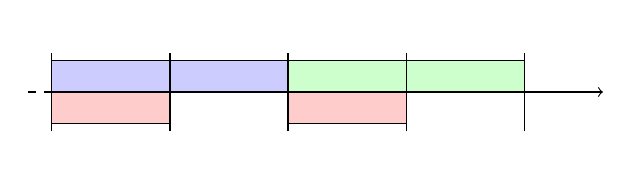
\begin{tikzpicture}
	
	\draw[->] (-.3, 0) -- (-.2,0) (-.1,0) -- (7,0);\node[] at (6.9,.2) {};
	
	\filldraw[fill=blue!20!white, draw=black] (0,0) rectangle (3,.4);
	\filldraw[fill=red!20!white, draw=black] (0,0) rectangle (1.5,-.4);
	\draw (0,-.5) -- (0,.5) (1.5,-.5) -- (1.5,.5);
	\draw[thick] (3,-.5) -- (3,.5);
	\filldraw[fill=green!20!white, draw=black] (3,0) rectangle (6,.4);
	\filldraw[fill=red!20!white, draw=black] (3,0) rectangle (4.5,-.4);
	\draw  (4.5,-.5) -- (4.5,.5);
	\draw  (6,-.5) -- (6,.5);
	
	\node[] at (.75,-.25) {}; \node[] at (.75,.2) {}; \node[] at (2.3,.2) {};
	\node[] at (1.65,.7) {}; \node[] at (.8,-.7) {};
	\node[] at (3.75,-.25) {}; \node[] at (3.75,.2) {}; \node[] at (5.3,.2) {};
	\node[] at (4.65,.7) {}; \node[] at (3.75,-.7) {};
	
	\end{tikzpicture}
	\caption{A general scenario which show how two subsequent  operations  and  can not return respectively  and  if  has been written before .}
	\label{fig:scenarioOrdering}
\end{figure}

\begin{theorem}\label{th:Garay}
	Let  be the algorithm in Fig. \ref{fig:server}-\ref{fig:client} and let .
	If  and  then  implements a MWMR Atomic register in the Garay's model.
	
\end{theorem}

\begin{proofT}
	It follows directly from Theorem \ref{t:termination}, \ref{t:validity} and \ref{t:ordering}.
	\renewcommand{\toto}{th:Garay}	
\end{proofT}

\begin{theorem}\label{th:Bonnet}
Let  be the algorithm in Fig. \ref{fig:server}-\ref{fig:client} and let .
	If  and  then  implements a MWMR Atomic register in the Bonnet's model.
\end{theorem}

\begin{proofT}
	It follows directly from Theorem \ref{t:termination}, \ref{t:validity} and \ref{t:ordering}.
	\renewcommand{\toto}{th:Bonnet}	
\end{proofT}

\begin{theorem}\label{th:Sasaki}
Let  be the algorithm in Fig. \ref{fig:server}-\ref{fig:client} and let .
	If  and  then  implements a MWMR Atomic register in the Sasaki's model.
\end{theorem}

\begin{proofT}
	It follows directly from Theorem \ref{t:termination}, \ref{t:validity} and \ref{t:ordering}.
	\renewcommand{\toto}{th:Sasaki}	
\end{proofT}

\begin{theorem}\label{th:Burhman}
Let  be the algorithm in Fig. \ref{fig:server}-\ref{fig:client} and let .
	If  and  then  implements a MWMR Atomic register in the Burhman's model.\end{theorem}

\begin{proofT}
	It follows directly from Theorem \ref{t:termination}, \ref{t:validity} and \ref{t:ordering}.
	\renewcommand{\toto}{th:Burhman}	
\end{proofT}

